\documentclass[conference]{IEEEtran}
\IEEEoverridecommandlockouts
\usepackage{amsmath,amssymb}
\usepackage{graphicx}
\usepackage{booktabs}
\usepackage{siunitx}
\usepackage{url}
\sisetup{detect-all}

\begin{document}

\title{Twist, Interpolation and Resolution Limits of\\
Curvature-Based Shape Sensing for Soft Continuum Arms}

\author{\IEEEauthorblockN{Anthony Ijoot}
\IEEEauthorblockA{Department of Electrical and Electronics Engineering\\
Makerere University, Kampala, Uganda\\
anthonyijoot98@gmail.com}}

\maketitle

\begin{abstract}
Soft continuum arms often estimate their shape by integrating curvature
measured by a few embedded sensors, yet the number of sensors, the
components they measure, the way their readings are interpolated and the
resolution of their converters are usually chosen by trial on a prototype.
We study these choices in simulation, where the true shape is known, for a
three-segment, \SI{25}{cm} elastomer arm under gravity and tip loads. A
static Kirchhoff rod model, cross-checked against the PyElastica Cosserat rod
simulator in tip position and twist, gives 400 equilibrium shapes; sensors
with a \SI{10}{mm} gauge, noise and quantization are placed along them, and
the shape is rebuilt by integrating the measured curvature. When twist is
not measured and is taken as zero, as kinematic reconstruction usually
assumes, the median tip error stays near 1.9\,\% of the arm length
(6.1\,\% at the 95th percentile) however many bending sensors are used,
because gravity and loads twist the arm; for a torsionally soft arm it
reaches 7.9\,\%. Measuring twist lowers it to 0.10\,\% with 12 sensors. The
constant-curvature-per-segment model stops at 0.6\,\% even with twist, and
interpolating within the actuated segments rather than across their
boundaries reduces it by a third to a half at 6 and 12 sensors. An error
model predicts the effect of noise and quantization to within 20\,\% and
shows that 11-bit conversion suffices when the sensors' own noise is below
\SI{0.006}{m^{-1}}; noisier sensors need fewer bits.
\end{abstract}

\begin{IEEEkeywords}
soft robotics, continuum robots, proprioception, shape sensing, Cosserat rod,
curvature sensors, twist, quantization
\end{IEEEkeywords}

\section{Introduction}

A soft continuum arm has no joints to encode. Its configuration is a curve,
and closed-loop control, contact estimation and teleoperation all need an
estimate of that curve from sensors carried by the arm itself
\cite{dellasantina2023survey}. Optical fibres with Bragg gratings, embedded
resistive or capacitive strain gauges and liquid-metal or ionic sensors all
report local strain, which a bending model turns into curvature
\cite{shi2017survey, galloway2019fiber}. The shape then follows by
integrating the curvature along the arm, the kinematics behind the
constant-curvature models of continuum robots \cite{webster2010review}.
Learned maps from many soft sensors to configuration
\cite{thuruthel2019perception, truby2020proprioception} and probabilistic
estimators that fuse a mechanical model with the measurements
\cite{lilge2022gp} are alternatives, but they too depend on what the sensors
can observe.

The designer of the sensing hardware faces coupled choices: how many sensors
to embed, which components of curvature they must measure, how to
interpolate between them, and how finely to digitize them. Each sensor costs
wiring, stiffness and an analog channel. Twist is a known difficulty in fibre
shape sensing, where measuring it needs helical or specially arranged
gratings \cite{xu2016helical}, but its effect on the shape of a soft arm
loaded by its own weight is rarely quantified, and the other choices are
usually settled on a prototype.

This paper studies these choices in simulation. Its contributions are: a
static rod model of a three-segment arm under gravity and tip loads,
cross-checked against a second simulator, used to produce 400 equilibrium
shapes; a sensing model with gauge averaging, noise and quantization, and
three reconstructions; the finding that twist, not sensor count, limits
kinematic reconstruction from bending-only sensors, and that the limit grows
as the arm becomes softer in torsion; a comparison of interpolation within
and across actuated segments; and an error model that gives the converter
resolution worth using for a given sensor count and noise.

\section{Arm Model}

\subsection{Static Kirchhoff rod}

Following the rod models used for continuum robots
\cite{rucker2011tendon, till2019realtime}, the arm is an inextensible,
unshearable rod of length $L$, clamped at the base with its tangent
horizontal. With arc length $s$, centreline $p(s)$, material frame $R(s)$
and body-frame curvature $u(s) = (u_1, u_2, u_3)$, where $u_3$ is the twist
of the material frame about the centreline,
\begin{equation}
p' = R\,e_3, \qquad R' = R\,\hat{u},
\label{eq:kin}
\end{equation}
with $\hat{u}$ the skew matrix of $u$. The internal force $n$ and moment
$m$, in the spatial frame, balance the distributed weight $f$:
\begin{equation}
n' + f = 0, \qquad m' + p' \times n = 0 .
\label{eq:eq}
\end{equation}
Actuation is modelled as an intrinsic bending curvature $u^*(s)$ that is
constant within each segment, as produced by pressurizing a segment's
chambers or pulling its tendons, with no intrinsic twist:
\begin{equation}
R^\top m = K\,(u - u^*), \qquad K = \operatorname{diag}(EI, EI, GJ).
\label{eq:const}
\end{equation}
The tip carries a force $F$ and no moment. The unknown base force and moment
are found by Newton's method on the tip conditions, integrating
(\ref{eq:kin})--(\ref{eq:const}) with 300 fourth-order Runge-Kutta steps and
ramping actuation and load in three steps. Each shape takes about
\SI{1.5}{s}.

\subsection{Parameters and cross-checks}

The arm is \SI{0.25}{m} long with a solid \SI{15}{mm} radius, density
\SI{1080}{kg/m^3} and an effective modulus of \SI{3}{MPa}, typical of a
fibre-reinforced elastomer; its own weight bends it \SI{30}{mm} downward
when unactuated. Three segments of equal length are actuated. For a solid
incompressible section $GJ/EI = 2/3$; Section~\ref{sec:twist} varies this
ratio.

The solver reproduces a circular arc exactly under pure intrinsic curvature,
and for a stiff rod under its own weight it matches the linear
Euler-Bernoulli tip deflection to five digits. It was also compared with
PyElastica \cite{gazzola2018filaments}, a dynamic Cosserat rod simulator that
includes shear and extension, damped to rest. The tip positions agree to
\SI{0.09}{mm} under gravity alone. With three-dimensional actuation, and with
a tip load added, they differ by 1.7 and \SI{1.2}{mm} (under 0.7\,\% of $L$)
with 240 PyElastica elements; in the first case the difference is 6.5, 3.3
and \SI{1.7}{mm} with 60, 120 and 240 elements, halving with each refinement
as the curvature steps at segment boundaries are resolved more finely. The
twist, the quantity central to this paper, agrees as well: with the tip load
the largest $u_3$ is 1.064 against \SI{1.050}{m^{-1}}, the rms difference
along the arm is \SI{0.002}{m^{-1}}, and the total twist is
\ang{-1.64} against \ang{-1.58}. The sensing study compares reconstructions
with shapes of the same rod model, so its conclusions do not rest on the
residual differences.

\subsection{Shape data set}

Each of 400 shapes draws, for every segment, a bending direction uniformly
in $[0, 2\pi)$ and an intrinsic curvature magnitude uniformly up to a
\ang{90} bend of the segment (\SI{18.8}{m^{-1}}). With probability one half,
213 of the 400 shapes, the tip also carries a force of random direction and
magnitude up to \SI{0.3}{N}, a sixth of the arm's weight, representing
contact or a payload. The median tip displacement from the straight arm is
0.68\,$L$ (Fig.~\ref{fig:shapes}). The largest bending curvature is
\SI{19.2}{m^{-1}}, and although actuation applies no twist, gravity and the
loads twist the arm by up to \SI{2.3}{m^{-1}}.

\begin{figure}[t]
\centering
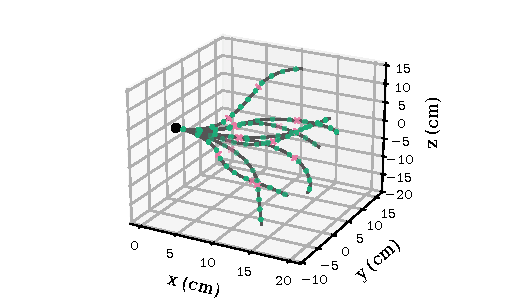
\includegraphics[width=\columnwidth]{fig_shapes.pdf}
\caption{Eight of the 400 equilibrium shapes. Base at the origin, tangent
along $x$, gravity along $-z$. Dots: 12 sensor positions; crosses: segment
boundaries.}
\label{fig:shapes}
\end{figure}

\section{Sensing and Reconstruction}

\subsection{Sensor model}

Sensor $j$, centred at $s_j = (j + \frac{1}{2})L/N$ with gauge length
$g = \SI{10}{mm}$, reports the exact average of the two bending curvatures
$(u_1, u_2)$ over its gauge; a three-axis sensor also reports the twist
$u_3$. White noise of rms $\sigma$ is added to every channel, and the result
is quantized with $B$ bits over $\pm\kappa_{\mathrm{fs}} =
\pm\SI{20}{m^{-1}}$, which covers every curvature in the data set. For
sensor counts that are multiples of three, every segment holds $N/3$
sensors and none sits on a segment boundary.

\subsection{Reconstruction}

The estimated curvature $\hat{u}(s)$ is integrated through (\ref{eq:kin})
from the clamped base. When twist is not measured it is set to zero, which
treats the sensors' frame as one that does not rotate about the centreline,
the usual assumption of kinematic shape reconstruction. Each integration
step applies the exact rotation of its constant curvature. Three estimates
of $\hat{u}$ are compared, all from the same sensor positions:
\begin{itemize}
\item \emph{one curvature per segment}: the mean of the segment's sensors,
held over the segment, the piecewise constant-curvature model
\cite{webster2010review};
\item \emph{across segments}: linear interpolation between neighbouring
sensors along the whole arm, held constant beyond the end sensors;
\item \emph{within segments}: linear interpolation between the sensors of a
segment only, held constant from the outermost sensor to the segment
boundary, so that changes of actuation at the boundaries are not smeared.
\end{itemize}
The last needs the segment boundaries, which the designer knows. Integrating
the true curvature, twist included, reproduces the true shape to 0.07\,\% of
$L$ at worst, the numerical floor of the comparison. Errors are reported as
the tip position error divided by $L$, as the median and 95th percentile
over the 400 shapes.

\section{Results}

\subsection{Twist limits bending-only reconstruction}
\label{sec:twist}

Fig.~\ref{fig:sensors} shows the tip error of ideal sensors against their
number. With bending-only sensors every reconstruction levels off at a
median of 1.9 to 2.2\,\% of $L$ (95th percentile 6.0 to 6.3\,\%), from 6
sensors up to 24. The cause is twist. Gravity acting on a
three-dimensionally bent arm, and any lateral tip force, twist the arm about
its own axis; a sensor fixed to the material then reports its curvature in a
frame that has rotated, and a reconstruction that ignores the rotation bends
the wrong way. Ignoring twist alone, with the bending curvature known exactly
everywhere, already produces a median of 1.9\,\%. Twist is not caused by the
tip loads alone: without them the median is 1.8\,\% and the 95th percentile
6.2\,\%. Measuring twist removes the floor: with 12 sensors the median falls
to 0.10\,\% and the 95th percentile to 0.17\,\%, about 19 and 36 times lower.

The floor depends on how easily the arm twists (Table~\ref{tab:twist}). With
$GJ/EI = 0.2$, as in a thin-walled or multi-chamber section, the
bending-only median rises to 7.9\,\% and the 95th percentile to 20\,\%; a
torsionally stiff, fibre-wound arm with $GJ/EI = 2$ still shows 0.8\,\%.
Three-axis sensing stays below 0.6\,\% at the 95th percentile in all three
cases. The two extra rows use 60 new random shapes each, so they compare
trends rather than identical poses.

The floor is a limit of kinematic integration, not of the information the
arm carries. The twist here comes from the torsional moment of gravity and
the tip load, so an estimator that combines the bending measurements with a
mechanical model of the arm and its loads \cite{lilge2022gp} could predict
much of it. Such an estimator needs the model and the loads; a twist
measurement needs neither.

\begin{figure}[t]
\centering
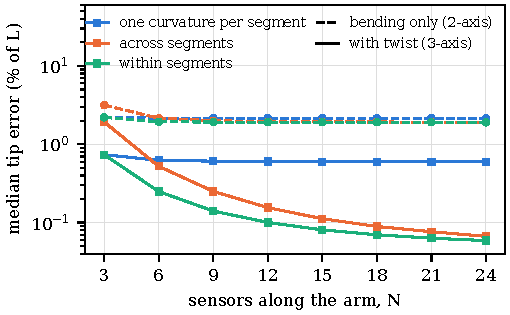
\includegraphics[width=\columnwidth]{fig_sensors.pdf}
\caption{Median tip error against the number of ideal sensors, for the three
reconstructions, with bending-only (dashed) and three-axis (solid) sensors.}
\label{fig:sensors}
\end{figure}

\begin{table}[t]
\caption{Tip error (\% of $L$, median / 95th percentile) with 12 ideal
sensors and interpolation within segments, against the ratio of torsional
to bending stiffness}
\label{tab:twist}
\centering
\begin{tabular}{@{}rrrcc@{}}
\toprule
$GJ/EI$ & Shapes & Max twist & Bending only & With twist \\
 & & (m$^{-1}$) & & \\
\midrule
0.2 & 60 & 8.3 & 7.89 / 20.27 & 0.19 / 0.58 \\
0.67 & 400 & 2.3 & 1.92 / 6.10 & 0.10 / 0.17 \\
2.0 & 60 & 0.8 & 0.79 / 2.09 & 0.08 / 0.10 \\
\bottomrule
\end{tabular}
\end{table}

\subsection{Constant curvature per segment is not enough}

With twist measured, one curvature per segment reaches 0.74\,\% with three
sensors and stops near 0.6\,\% however many sensors are averaged
(Fig.~\ref{fig:sensors}). Under gravity and tip loads the curvature varies
along each segment, because the bending moment of the weight and the load
grows towards the base, and a constant-curvature model cannot represent the
variation.

\subsection{Interpolating within segments}

Linear interpolation follows the variation, but it matters where it is
allowed to act. Interpolating across a segment boundary smears the change of
actuation there over a sensor spacing; interpolating within segments keeps
it. From the same sensor positions the median error falls from 0.52 to
0.25\,\% with 6 sensors, from 0.25 to 0.14\,\% with 9 and from 0.16 to
0.10\,\% with 12; beyond 15 sensors both approach about 0.06\,\%. The
benefit does not depend on the actuation changing abruptly: when the
intrinsic curvature changes linearly over \SI{20}{mm} at each boundary (200
further shapes), the median falls from 0.46 to 0.28\,\% with 6 sensors and
from 0.19 to 0.11\,\% with 12, though hardly at all with 9 or 24.

\subsection{Gauge length}

The gauge length hardly matters. From 2 to \SI{20}{mm} the median error with
12 three-axis sensors stays between 0.09 and 0.10\,\%, and with 6 sensors
between 0.23 and 0.25\,\%: within a segment the curvature varies slowly
enough that a long stretchable gauge loses nothing against a short one.

\subsection{Resolution and noise}

A curvature error held over the sensor spacing $L/N$ at arc length $s$
tilts the rest of the arm and moves the tip by about $(L-s)\,L/N$ times the
error. If each sensor carries an independent error of rms $\sigma_e$ on each
bending axis, summing over sensors and two axes gives
\begin{equation}
\frac{e_{\mathrm{rms}}}{L} \approx
\sqrt{\left(\frac{e_0}{L}\right)^{2} + \frac{2}{3}\,\frac{\sigma_e^{2} L^{2}}{N}},
\qquad \sigma_e^2 = \sigma^2 + \frac{q^2}{12},
\label{eq:model}
\end{equation}
where $q = 2\kappa_{\mathrm{fs}}/2^B$ is the quantization step and $e_0$ the
error with ideal sensors, taken from the simulation. The model neglects the
error on the twist channel and uses the straight-arm lever arm $L - s$,
which overstates the lever of a curved arm; the two partly cancel.
Fig.~\ref{fig:bits} compares (\ref{eq:model}) with the simulated rms error
for 6, 12 and 24 sensors. At 8 and 10 bits, and for white noise of 0.05 and
\SI{0.2}{m^{-1}}, the model is within 20\,\%. At 6 bits with 24 sensors it
underestimates the error by a third: the gauges then nearly touch,
neighbouring sensors see almost the same curvature, and their quantization
errors are no longer independent.

The quantization term halves with each bit while $e_0$ falls only as sensors
are added, so each sensor count has a resolution beyond which bits are
wasted. Table~\ref{tab:bits} lists the fewest bits that keep the 95th
percentile within 20\,\% of its ideal-sensor value for noise-free sensors:
8 bits for three sensors, 10 for six to nine and 11 for twelve or more. At
8 bits, 12 sensors give a median of 0.24\,\%, 2.4 times their ideal value.
These counts hold only while the sensors' own noise is below the
quantization noise, about \SI{0.006}{m^{-1}} at 11 bits. Real soft sensors
are often noisier: white noise of \SI{0.05}{m^{-1}} rms, a quarter of a
percent of the full-scale value, costs as much as 8-bit quantization (a
median of 0.24\,\% with 12 sensors). With such sensors, (\ref{eq:model})
shows that bits beyond the point where $q/\sqrt{12}$ falls below $\sigma$
buy little, and lowering the noise or adding sensors is what helps.

\begin{figure}[t]
\centering
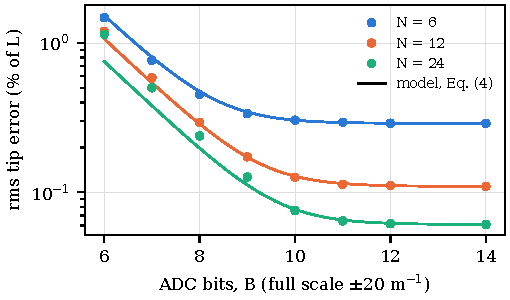
\includegraphics[width=\columnwidth]{fig_bits.pdf}
\caption{Rms tip error against converter resolution for noise-free
three-axis sensors interpolated within segments. Dots: simulation; lines:
the model (\ref{eq:model}).}
\label{fig:bits}
\end{figure}

\begin{table}[t]
\caption{Fewest bits keeping the 95th-percentile tip error within 20\,\% of
the ideal-sensor value (noise-free three-axis sensors, interpolation within
segments, full scale $\pm\SI{20}{m^{-1}}$)}
\label{tab:bits}
\centering
\begin{tabular}{@{}rccc@{}}
\toprule
Sensors $N$ & Ideal 95th pct. & Bits & 95th pct. at those bits \\
 & (\% of $L$) & & (\% of $L$) \\
\midrule
3 & 1.33 & 8 & 1.45 \\
6 & 0.46 & 10 & 0.50 \\
9 & 0.25 & 10 & 0.27 \\
12 & 0.17 & 11 & 0.17 \\
18 & 0.11 & 11 & 0.12 \\
24 & 0.09 & 11 & 0.10 \\
\bottomrule
\end{tabular}
\end{table}

\section{Discussion}

\emph{Design guidance.} For an arm of this kind the results suggest an order
of priorities. First, account for twist: measure it, for instance with
helically arranged gauges or gratings \cite{xu2016helical}, build the arm
stiff in torsion, or estimate it with a model of the arm and its loads.
Second, interpolate within the actuated segments rather than across their
boundaries, and avoid the constant-curvature model when gravity or loads are
significant. Third, choose the converter from (\ref{eq:model}) and the
measured sensor noise. With twelve noise-free three-axis sensors at 11 bits
the tip stays within 0.17\,\% of the length, \SI{0.4}{mm} on this arm, for
95\,\% of the shapes.

\emph{Scope.} The study is a simulation of one arm. The rod is static,
inextensible and isotropic in bending; real elastomer arms also extend under
pressure, may couple actuation to twist, creep and show hysteresis, and real
sensors drift with temperature and couple bending to strain. A real twist
channel is likely to be noisier than a bending channel, which
(\ref{eq:model}) does not include. The tip loads are applied forces rather
than contact, and dynamics are not considered. The numbers therefore
describe how the error scales with the sensing choices rather than the
accuracy of a particular prototype; the next step is to measure the
predicted twist floor and interpolation gain on a fabricated arm with motion
capture.

\section{Conclusion}

Kinematic reconstruction of a soft arm's shape from embedded curvature
sensors is limited by what the sensors miss before it is limited by how many
there are. Bending-only sensors leave errors of about 2\,\% of the length on
a solid elastomer arm and 8\,\% on a torsionally soft one, because gravity
and loads twist the arm. Measuring twist lowers the error by more than an
order of magnitude, interpolating within actuated segments lowers it by a
further third to a half at small sensor counts, and a simple error model gives
the converter resolution beyond which, for a given sensor noise, more bits
buy nothing.

\begin{thebibliography}{99}

\bibitem{dellasantina2023survey}
C.~Della Santina, C.~Duriez, and D.~Rus, ``Model-based control of soft
robots: A survey of the state of the art and open challenges,'' \emph{IEEE
Control Syst. Mag.}, vol.~43, no.~3, pp.~30--65, 2023.

\bibitem{shi2017survey}
C.~Shi, X.~Luo, P.~Qi, T.~Li, S.~Song, Z.~Najdovski, T.~Fukuda, and H.~Ren,
``Shape sensing techniques for continuum robots in minimally invasive
surgery: A survey,'' \emph{IEEE Trans. Biomed. Eng.}, vol.~64, no.~8,
pp.~1665--1678, 2017.

\bibitem{galloway2019fiber}
K.~C. Galloway, Y.~Chen, E.~Templeton, B.~Rife, I.~S. Godage, and E.~J.
Barth, ``Fiber optic shape sensing for soft robotics,'' \emph{Soft Robot.},
vol.~6, no.~5, pp.~671--684, 2019.

\bibitem{webster2010review}
R.~J. Webster~III and B.~A. Jones, ``Design and kinematic modeling of
constant curvature continuum robots: A review,'' \emph{Int. J. Robot. Res.},
vol.~29, no.~13, pp.~1661--1683, 2010.

\bibitem{thuruthel2019perception}
T.~G. Thuruthel, B.~Shih, C.~Laschi, and M.~T. Tolley, ``Soft robot
perception using embedded soft sensors and recurrent neural networks,''
\emph{Sci. Robot.}, vol.~4, no.~26, art.~eaav1488, 2019.

\bibitem{truby2020proprioception}
R.~L. Truby, C.~Della Santina, and D.~Rus, ``Distributed proprioception of
3D configuration in soft, sensorized robots via deep learning,'' \emph{IEEE
Robot. Autom. Lett.}, vol.~5, no.~2, pp.~3299--3306, 2020.

\bibitem{lilge2022gp}
S.~Lilge, T.~D. Barfoot, and J.~Burgner-Kahrs, ``Continuum robot state
estimation using Gaussian process regression on SE(3),'' \emph{Int. J.
Robot. Res.}, vol.~41, no.~13--14, 2022.

\bibitem{xu2016helical}
R.~Xu, A.~Yurkewich, and R.~V. Patel, ``Curvature, torsion, and force
sensing in continuum robots using helically wrapped FBG sensors,''
\emph{IEEE Robot. Autom. Lett.}, vol.~1, no.~2, pp.~1052--1059, 2016.

\bibitem{rucker2011tendon}
D.~C. Rucker and R.~J. Webster~III, ``Statics and dynamics of continuum
robots with general tendon routing and external loading,'' \emph{IEEE Trans.
Robot.}, vol.~27, no.~6, pp.~1033--1044, 2011.

\bibitem{till2019realtime}
J.~Till, V.~Aloi, and C.~Rucker, ``Real-time dynamics of soft and continuum
robots based on Cosserat rod models,'' \emph{Int. J. Robot. Res.}, vol.~38,
no.~6, pp.~723--746, 2019.

\bibitem{gazzola2018filaments}
M.~Gazzola, L.~H. Dudte, A.~G. McCormick, and L.~Mahadevan, ``Forward and
inverse problems in the mechanics of soft filaments,'' \emph{R. Soc. Open
Sci.}, vol.~5, art.~171628, 2018.

\end{thebibliography}

\end{document}
